\section{Shading}

Shading is a way of giving the perception of depth in 3D illustrations.
This is achieved by depicting levels of darkness with respect to a given
light source. This section will attempt to describe to kinds of shading used
in computer graphics, flat and Phong shading. Each section will consist of a
short description of the overall theory behind the shading method followed by a
quick mention of our implementation.

\subsection{Que?}

\subsection{Flat shading}

\subsection{Phong shading}
Flat shading is a little brutal, especially with respect to specularity. If a
surface has large specular areas they will either be ignored, or define the
intensity of the entire surface. Phong illumination corrects this problem.

\begin{figure}[hbt]
	\centering
	\scalebox{0.5}
	{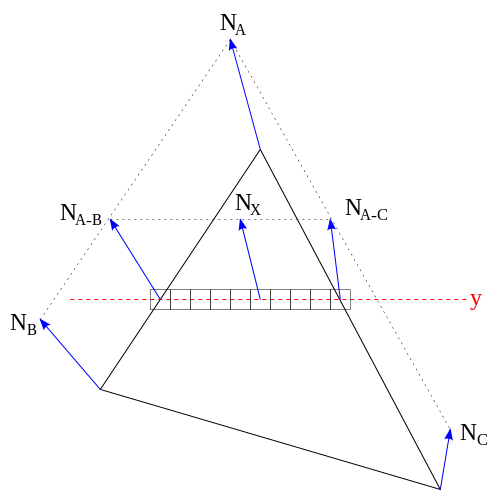
\includegraphics{pics/phongInterpol.png}}
	\caption{Normal interpolation in Phong shading}
	\label{fig:phongInterpo}
\ref{fig:phongInterpo}
\end{figure}

By interpolating the vertex normals across the polygon surface (figure
\ref{fig:phongInterpo}), Phong shading finds a smoothly shifting normal for each
pixel. This normal is then used in the illumination/reflection model, to find
the final intensity weight for that pixel. This will give a much more realistic
result that flat shading, at the expense of interpolating normals and applying
the lighting model for each surface pixel. Figure \ref{fig:fVsP} illustrates
both the improved colour realism (the sphere actually looks spherical), and the
difference in specularity, being completely invisible in the example using flat
shading.

\begin{figure}[htb]
	\centering
	\scalebox{0.7}
	{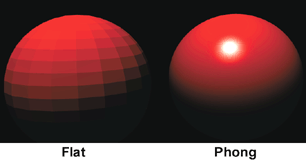
\includegraphics{pics/flatVsPhong.png}}
	\caption{flat vs Phong shading}
	\label{fig:fVsP}
\ref{fig:phongInterpo}
\end{figure}

\subsection{Estimating the point of impact}
Estimating a point of impact. 
One of the main obstacles we faced while programming the Phong shading model, was determining the exact points in world coordinates on which the light hit the box surface. This point is needed for correct visualization of both the diffuse and the specular lighting. As a bad estimate we started out just by using the center point for each surface, but the results gained from this method were not impressive. Instead we tried to utilize that we had some known points on each surface, trying to estimate some points in between to use in a more realistic lighting model. 
Instead of iterating through the pixels of each surface, we iterate through the 10x10 shadeRes matrix. Each point in 2d here corresponds to a 3d point on the box surface. (Note that we also experienced a bit with using a homography from the box surface in 3d to a 2d coordinate system, in effect doing an inverse projection, but instead we decided to estimate it the other way around).
As our 2d coordinate system in this case is 10x10  each surface determines the vector from the center to one of the corner points. This vector is divided by 5 to get the increment factor of each axis. This factor times ten (each axis x,y,z fully incremented) gives us the opposite corner point. Each time we increment either of the axis (x or y) in  our 2d coordinate system, we increment each axis accordingly in our 3d world coordinate system adding the value to our start/corner coordinate, thus allowing us to iterate through each surface on the box. The new light vector is then calculated from the light source to the surface point in world coordinates. 
